
%---Define your document class, packages, and new commands

\documentclass[11pt]{article}
\usepackage[top=2.54cm, left=2.54cm, right=2.54cm, bottom=2.54cm]{geometry}

\usepackage{amsfonts}   % for statements to be commented out
\usepackage{amssymb}
\usepackage{amsmath}    % for subequations
\usepackage{setspace}
\usepackage{graphicx}


%------------Document-Begins-Here----------------------%

\begin{document}


\title{\textbf{Orbital Patterns of Martian Moons}}

\author{Jake Mathews
\thanks{mathewsj2@wit.edu}\\
Computer Science Undergraduate Program, Wentworth Institute of Technology\\
550 Huntington Avenue, Boston, MA 02115\\
\and Ian Brown
\thanks{browni1@wit.edu}\\
INSERT MAJOR HERE, Wentworth Institute of Technology\\
550 Huntington Avenue, Boston, MA 02115}

\maketitle

\begin{abstract}

This project's goal was to to create a top-down 2-dimentional model
of the positional path of the moons of Mars, Phobos and Deimos.
We created a Fortran 90 program to simulate the orbit of the two moons
and generate data files for later analysis.
The simulation will be provided some initial conditions of a given moon,
and simulate the orbit over the course of one orbital period, as defined
by NASA~\cite{nasa}

\end{abstract}




% Write your introduction here, include pictures, tables, equations, etc...
\section{Introduction}
An object in orbit is a simple kinematics problem illustrated in Fig.~\ref{fig:centripetal}

\begin{figure}[ht]
  \centering
  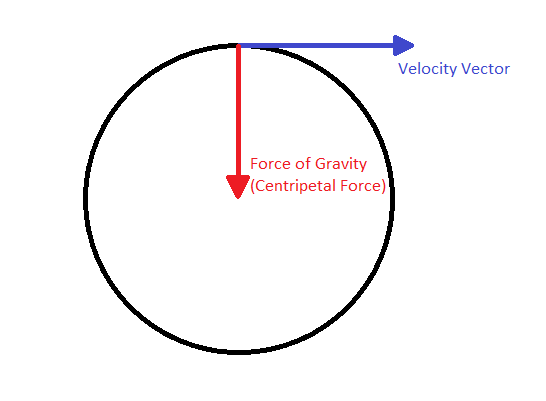
\includegraphics[width=0.6\textwidth, angle =0]{../images/centripetal-force}
  \caption{Centripetal force on an object with a velocity vector}
  \label{fig:centripetal}
\end{figure}
\noindent
In Fig.~\ref{fig:centripetal} there is an object with an intial velocity vector
and a centripetal force pulling it towards the center. The black circle represents
the objects path over time. In the case of an orbit, the velocity vector is always 
perpendicular to the centripetal force vector. This is what the program is attempting to simulate,
where the orbiting object is each of the Mars' moons, the center object is Mars
iteself, and the centripetal force providing the acceleration to change each moon's
velocity vector is gravity.

\vspace{\baselineskip} \noindent
The program will need some initial conditions to be set before simulating
the motion of Phobos and Deimos such as the initial position, the initial
velocity, moon mass, Mars mass, gravitational constants, as well as time steps and a maximum 
simulation period. Initial velocity and gravitational constants are calculated
by the program based of the properties in Table~\ref{table:moon-properties}.

\begin{table}[ht]
  \centering
  \begin{tabular}{|r|c|c|}
  \hline
  Moon Orbit Properties                & Phobos  & Deimos  \\ \hline
  Semi-Major Axis ($km$)                 & 9378    & 23459   \\ \hline
  Mass ($10^{15} kg$) & 1015    & 2.4     \\ \hline
  Orbital Period ($Earth\ days$)          & 0.31891 & 1.26244 \\ \hline
  \end{tabular}
  \label{table:moon-properties}
  \caption{Properties of Phobos and Deimos as described by NASA~\cite{nasa}}
  \end{table}

\noindent
The initial $x-y$ position is defined by each moons semi-major axis. 
The semi-major axis is half the length of the major axis of an ellipse.
This is illustrated in Fig.~\ref{fig:semi-major-axis} with both 
Phobos and Deimos labled.

\begin{figure}[ht]
  \centering
  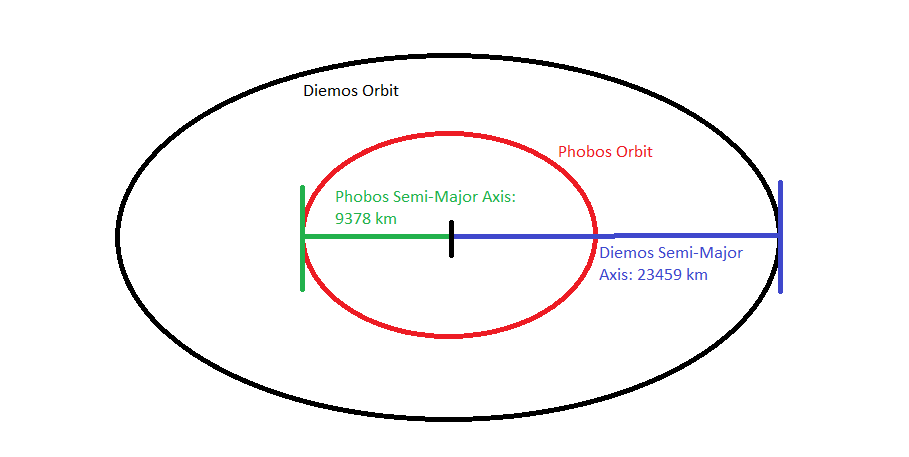
\includegraphics[width=1.0\textwidth, angle =0]{../images/semi-major-axis}
  \caption{A depiction of the semi-major axis of both Phobos and Demimos}
  \label{fig:semi-major-axis}
\end{figure}




% Do ALL math derivations here...label each equation and reference the
% equations accordingly... For example:  From Eq. (2), we see that Eqs. (3) - (7) 
% can be simplified, blah, blah...
\section{Theory}
\noindent For every equation, you need to explain each variable, for example:

\begin{equation}
\label{eq:force}
F=\dfrac{mv^2}{r}~.
\end{equation}
\noindent In Eq.~\eqref{eq:force}, $F$ is the force measured in Newtons, $m$ is the
mass in kilograms, $v$ is the velocity measured in meters per second, and $r$ is
the radius of the curved path.  Equation~\eqref{eq:force} was obtain from~\cite{uni}.




\section{Computational Methods \& Techniques}
\noindent Include snipits of your code, DO NOT INCLUDE YOUR ENTIRE CODE HERE!!!!  
Write about the methods you used, make sure you \textbf{\textit{explain}} the methods!!  Don't
just say we used ``RK4", you need to explain what is RK4.

\section{Results}
\noindent Include ALL results here, including tables of results, plots of results, numerical values, etc...
Make sure you include a figure caption for EACH figure.  Make sure you include a table caption for each table.
For example:
\begin{figure}[ht]
\centering
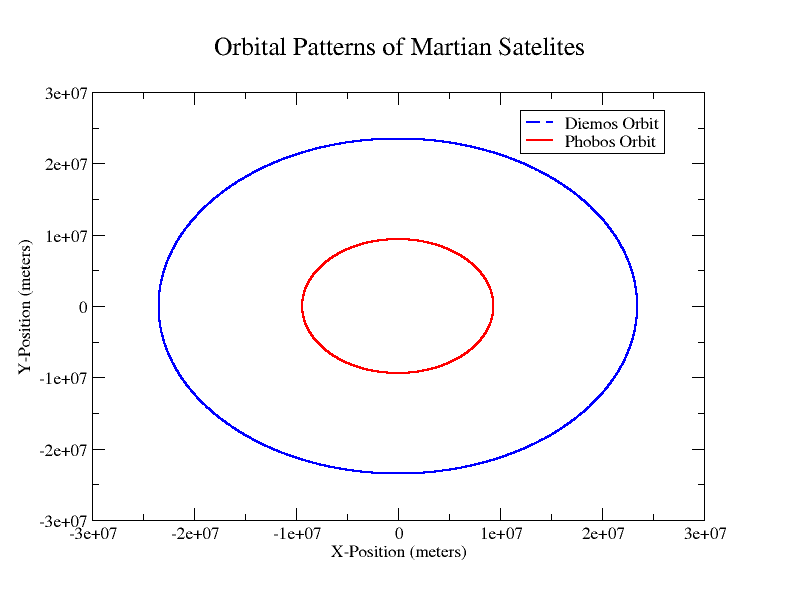
\includegraphics[width=1.0\textwidth, angle =0]{../images/orbits}
\caption{Orbital period in the $x-y$ plane for one full orbit of Phobos and Deimos orbiting Mars.}
\label{fig:orbit-diagram}
\end{figure}
\noindent In Fig.~\ref{fig:orbit-diagram}, the orbit is set to 2 full periods...

\section{Conclusions}
\noindent Summarize your results...This should be about a 1 page minimum!!!




\begin{thebibliography}{99}

\bibitem{uni} 
Douglas C. Giancoli
\textit{Physics for Scientists and Engineers}. 
Pearson Education Inc., Upper Saddle River, New Jersey, 2009.

\bibitem{nasa} 
NASA
\textit{Mars Fact Sheet}. 
NASA, 2016
nssdc.gsfc.nasa.gov/planetary/factsheet/marsfact.html

\end{thebibliography}




\end{document}